\section{Related Work}

\subsection{\cite{LabelingLanguageLearning}: In-Situ Labeling for Augmented Reality Language Learning}
%Huynh-2019 In-Situ Labeling for Augmented Reality Language Learning.
\cite{LabelingLanguageLearning} schaffen ein Framework, mit dem die Lernmethode 'loci' in Augmented Reality umgesetzt und erweitert werden kann. Die Lernmethode beruht darauf, Gegenstände der Welt mit Notizen zu beschriften. Dafür wurde folgende automatische Real-Time Objekt Erkennung entwickelt: Mithilfe von Image Based Object Detection werden Objekte auf RGB-Fotos der AR Umgebung erkannt. Diese Objekte werden dann in die 3D Szene der Umgebung übernommen. 

Die AR Brille hat zu wenig Rechenleistung, um Image Based Object Detection durchzuführen, daher wurde eine Server-Client Architektur aufgesetzt. Die Videokamera der AR Brille nimmt ein Video der Umgebung auf, das dann frameweise an den Server geschickt werden. Die einzelnen Frames werden an den Server geschickt. Dieser nutzt ein neuronales Netzwerk, um alle erkennbaren Objekte in dem Bild zu finden und mit Bounding Boxen zu lokalisieren.

Die ObjectDetection API von TensorFlow wird verwendet. Es findet mehrere Objekte in einem Foto in einer Analyse und gibt Bounding Boxen an. Die Objekterkennung soll in Real-Time durchgeführt werden. Um die Laufzeit dieser möglichst gering zu halten, wird die niedrigste Kameraauflösung mit 896x504 Pixel verwendet und die Fotos werden als JPEG komprimiert. Damit braucht die Analyse 30 ms pro Foto. Dies ermöglicht eine Real-Time Erkennung mit 30 Frames pro Sekunde. Trotzdem ist die Erkennung in der Applikation durch einen Netzwerk Delay von 150 ms zwischen der Hololens und dem Server verspätet.

Die Hololens nummeriert die Frames, die an den Server geschickt werden. Zusätzlich wird für jedes Frame die Kameraposition gespeichert, mit der es aufgenommen wurde. So können Frames asynchron analysiert werden. Ist die Analyse durchgelaufen, werden die Bounding Boxen der Objekte und die Kameraposition genutzt, um die Objekte in der 3D Umgebung zu lokalisieren. Dafür wird der Mittelpunkt jeder Bounding Box mithilfe eines Raycastes in die 3D Szene projiziert.

Ein Objekt wird erst markiert, wenn es auf mehreren Fotos gefunden wurde, um Fehlern bei der Objekterkennung entgegenzuwirken. Durch die Analyse des ersten Fotos wird eine ungefähre Position in der AR Umgebung für das Objekt ermittelt. Dieses Objekt wird dann mit den Objekten verglichen, die während der nächsten 60 Frames erkannt wurden. Haben die Objekte dieselbe semantische Bedeutung und eine ähnliche Position in der AR Umgebung, wird davon ausgegangen, dass es sich um ein einziges Objekt handelt, welches in den 60 Frames mehrmals aufgenommen wurde. Siehe Abbildung \ref{img:60frames}.

\begin{figure}[H]
	\centering
	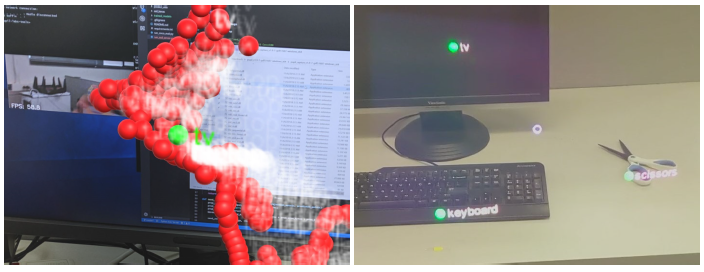
\includegraphics[width=0.8\textwidth]{images/img_huynh.PNG}
	\caption[Objekterkennung von \cite{LabelingLanguageLearning}]{Ungefähre Positionen des Objektes über 60 Frames aufgenommen in rot. Finale Position in grün.\citep{LabelingLanguageLearning}}
	\label{img:60frames}
\end{figure}

Unser Vorgehen zur Objekterkennung ähnelt dem Framework von \cite{LabelingLanguageLearning}. Auch hier soll die AR Umgebung durch das Hinzufügen von Labels semantisch angereichert werden. Es wird ebenfalls ein neuronales Netz verwendet, um die Object Detection auf RGB-Bildern durchzuführen. Wir haben dafür keinen eigenen Server aufgesetzt, sondern nutzen einen Cloud Service von Microsoft Azure. Durch Abspeichern von erhobenen semantischen Informationen ist eine Real-Time Detektion nicht relevant. Daher kann die Bild-Analyse länger dauern, was es erlaubt, mehrere neuronale Netze zu verwenden, die nach unterschiedlichen semantischen Informationen suchen.

In unserem Verfahren werden erkannte Objekte schon in der Umgebung markiert, wenn sie ein einziges Mal erkannt wurden. Wenn das Objekt erneut aufgenommen wird, wird die neue Analyse dem Objekt die gleiche Klasse und eine ähnliche Position der AR Umgebung zuweisen. Daran lässt sich erkennen, das es sich um dasselbe Objekt handelt.

Die erste Position, die für das Objekt berechnet wurde und die Position, die aus der zweiten Aufnahme hervorgeht, unterscheiden sich mit hoher Wahrscheinlichkeit ein wenig voneinander. Daher werden die Positionen gemittelt, um eine akkuratere Position für das Label des Objektes zu finden. 
\citep{LabelingLanguageLearning}

%todo Die related work ist noch zu Kompakt - hier solltest du auch mehr über view management reden, und text labels - das paper von Bell ist schon was alt, da gibt es viel neues. Zb. mal schauen beim Joe Gabbard und Markus Tatzgern. Du solltest das kapitel vielleicht auch anfangen mit ein kurzen übersicht / zusammenfassung. 

\subsubsection{View Management}

In Augmented Reality Anwendungen werden häufig Objekte der realen Welt durch Labels mit Informationen annotiert. Die Labels können entweder 3D Elemente oder 2D Elemente sein, die sich auf der Bildebene befinden. Ein Text-Label ist ein Schriftzug, der über eine Leader Line mit einem Anchor verbunden ist. Der Anchor gibt die Position des Objektes in der Szene an, das durch das Label beschriftet wird.

View Management ist das erstellen eines Layouts für die Labels. Das Ziel besteht darin die Labels gut lesbar auf der Bildebene zu positionieren und darzustellen. Dazu gehört, dass Labels sich gegenseitig nicht verdecken und auf eine verständliche Weise mit ihren Anchors verbunden sind. Einige View Management Vorgehen legen auch Wert darauf, relevante Objekte oder Regionen der realen Welt zu bestimmen, die reich an Informationen sind, oder für eine gegebene AR Anwendung relevant sind. Diese Bereiche der realen Welt sollen nicht durch Labels verdeckt werden.

Die Umsetzung von View Management unterscheidet sich je nachdem, ob die Labels 3D Elemente oder 2D Elemente sind. Für beide Typen sind die Ziele jedoch gleich. Es gibt viele Vorgehensweisen, um View Management umzusetzen. Weiterhin unterscheiden sich die Vorgehensweisen darin, ob sie Wissen über die Geometrie der Szene nutzen (Geometry Based) oder Fotos der Bildebene verwenden (Image Based).

%greedy algorithmn oder force based algorithm werden eingesetzt, oder lerning based algorithms.

\citep{viewManagementGrasset} stellen ein Image based View Management Vorgehen für 2D Labels vor. Das Verfahren wird eingesetzt um Gebäude und Plätze der realen Welt mit 2D Labels zu beschriften. Mit einer Aufnahme der Bildebene wird eine Saliency Mag erzeugt. Diese gibt die Einzigartigkeit jedes Pixels an. Diese Map wird mit einer Kantendetektion kombiniert, um eine Importance Map zu erstellen. Diese gibt an, wie Informationsreich die Pixel sind. Mit dieser Map als Grundlage wird entscheiden, in welchem Bildbereichen Labels gesetzt werden können und welche vermieden werden sollten.

Es wurde eine Menge an Funktionen aufgestellt, mit denen die optimale Position eines Labels gefunden werden kann. Jede Funktion berechnet eine Wertung für ein gegebenes Label und eine Position der Bildebene im Hinblick auf die unterschiedlichen Ziele, die das Layout erfüllen soll. Dazu gehört, dass gewisse Bereiche der Importance Map und der Kantendetektions Map vermieden werden und dass Labels sich gegenseitig nicht verdecken sollen. Darüber hinaus soll die Distanz zwischen einem Label und seinem Anchor minimiert werden und es kann eine favorisierte Richtung für die Leader Line angegeben werden, die den Look des Layouts beeinflussen kann. Mit einem Greedy Algorithmus wird die Position des Displays gefunden, an dem die Ziele, laut den Funktionen am besten erfüllt sind.
%springen von Labels?

%Um das Springen von Labels minimieren wird die berechnung des layouts mit einer nierigen frequenz ausgeführt. Die Labels werden nur an eine neue position gewegt, wenn sie besser ist als die alte und die labels werden mit einer smoothen animation zwischen positionen transitioned.

Zusätzlich zu dem Layout, das die Positionen der Labels bestimmt, wird das Aussehen der Labels an ihren Hintergrund adaptiert damit sie lesbar sind. Beispielweise erhalten die Leader Lines eine unterschiedliche Farbe abhängig von den Farben der Bildregionen, auf denen sie liegen.\cite{viewManagementGrasset} %Der Schriftzug eines Text-Labels hat ein background ein einen Background geben dessen lightness adaptiv ist. 


%für Augmented Reality Brower eine View Management Vorgehen entwickelt, das nicht darauf beruht, viel wissen über die Szene zu haben. 
%Vorgeben analysiert Video bilder um das Placement von Labels zu bestimmen und das Aussehen der Labels zu modifizieren.
%Labels so platziert, das wichtige infomration der realen Welt nicht versteckt wird, die Labels gut mit den objekten die sie annotieren sollen zusammenbleiben  und lesbarkeit der labels machen.
%
%
%
%
%
%
%andere works: geometry based layout oder image based layout
%
%geometrich based layout. haben wissen über den geometrischen aufbau der szene. ignorieren den view von realen objekten. beispiel davon ist Bell et al. 
%
%geometric based layout. layout of point features in goegraphic information systems and catography. NP hard problem. combined with image analysis. 
%
%image based layout
%learning based approcha um gute regionen zu finden in denen in AR ein Label platziert werden kann. Importance Maps aus video bildern. kann auch contraints an die positoinen der labels geben und dynamische labels machen.
%


%<old>
%
%\cite{viewmanagement3d} beschreiben View Management für interaktive 3D Benutzeroberflächen. Als View Management wird die Positionierung von Labels bezeichnet.
%Die Labels können sich auf eine 2D Ebene beschränken oder im 3D Raum liegen. View Management zielt darauf ab die Labels so zu positionieren, dass sie einander und relevante reale Objekte nicht verdecken. Gleichzeitig sollen die Labels die Gegenstände der realen Welt auf eine verständliche Art annotieren. Labels sollen nahe bei den Objekten liegen, zu denen sie gehören. Siehe Abbildung \ref{viewManagement}.
%
%\begin{figure}[H]
%	\centering
%	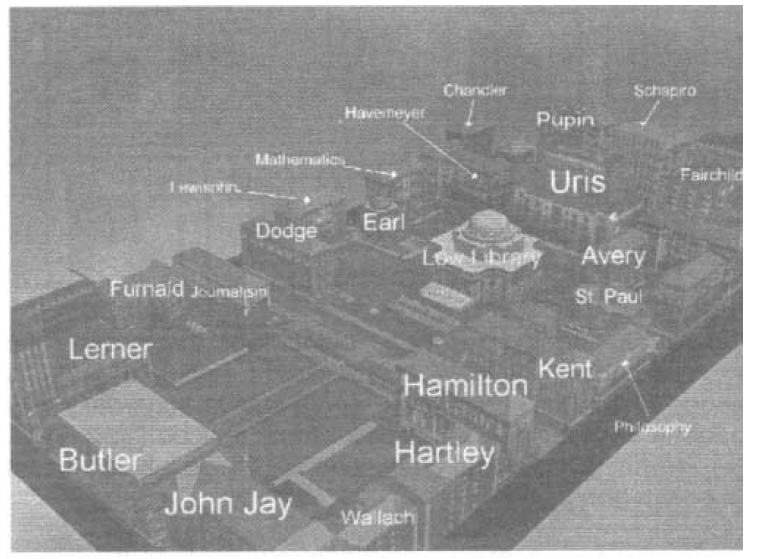
\includegraphics[width=0.7\textwidth]{images/img_viewmanagement.PNG}
%	\caption[View Management von \cite{viewmanagement3d}]{3D Labels durch View Management positioniert.\citep{viewmanagement3d}}
%	\label{viewManagement}
%\end{figure}



Unsere Applikation würde durch View Management profitieren. Nachdem Gegenstände in der Umgebung erkannt wurden, werden sie in dem 3D Raum durch 3D Labels markiert. Die Lesbarkeit dieser Labels kann durch View Management verbessert werden, indem ihre Positionen über Zeit verändert werden. 

Es müsste auf Veränderungen des Betrachtungswinkels und auf Hinzukommen von neuen Labels reagiert werden. Idealerweise würden die Labels einander und zusätzlich die Gegenstände der realen Welt nicht verdecken, die mit einem Label annotiert sind. 

View Management geht jedoch über den Rahmen dieser Arbeit hinaus und konnte nicht umgesetzt werden. %\citep{viewmanagement3d,viewmanagement}



\subsection{\cite{contextawaremixedreality}: Context-Aware Mixed Reality: A Framework for Ubiquitous Interaction}

\cite{contextawaremixedreality} stellen ein Framework vor, das einer AR Umgebung semantische Eigenschaften zuweist, um realistische Interaktionen zwischen virtuellen und realen Objekten zu erreichen. 
Insbesondere sollen physikalische Interaktionen an Realismus gewinnen.

Das Framework reichert die Umgebung mit Informationen über die Materialien an, aus denen reale Oberflächen und Gegenstände in der Umgebung bestehen. Die Umgebung wird in einer 3D Szene durch ein Mesh repräsentiert. Die einzelnen Voxel des Meshes werden mit Labels annotiert, um ihnen Semantik zuzuweisen.

Als beispielhafte Applikation wurde ein First-Person-Shooter vorgestellt, bei dem das Aussehen von Einschusslöchern davon abhängt auf welches Material geschossen wurde. Siehe Abbildung \ref{img:game}.

\begin{figure}[h]
	\centering
	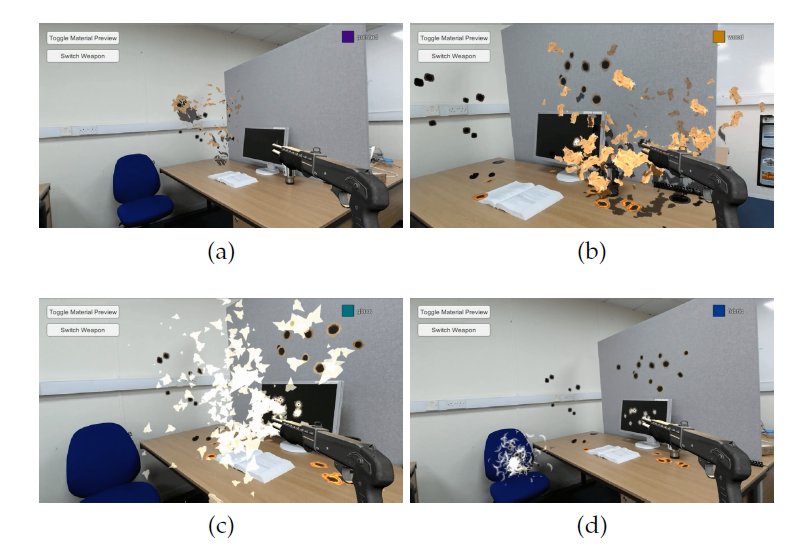
\includegraphics[width=0.8\textwidth]{images/img_shootinggame.png}
	\caption[Context Aware Shooter von \cite{contextawaremixedreality}]{Es gibt unterschiedliche Interaktionen, wenn auf eine Wand (a), einen Tisch (b), einen Bildschirm (c) und einen Stuhl (d) geschossen wird.\citep{contextawaremixedreality}}
	\label{img:game}
\end{figure}

Für die Erkennung der Materialien werden mehrere Frames der Hololens segmentiert. Die dadurch entstehenden semantischen Informationen werden abgespeichert, um bei späteren Interaktionen der AR Applikation abgerufen werden zu können. Die Erkennung der Materialien ist nicht echtzeitfähig, aber durch das Speichern der Materialien im Raum können die Interaktionen in Echtzeit ablaufen. Die semantischen Informationen müssen nicht mit jedem Frame bestimmt werden.

RGB-Bilder der Umgebung werden aufgenommen und mit einem neuronalen Netzwerk analysiert, um semantische Informationen zu erheben. Das neuronale Netz wurde von \cite{contextawaremixedreality} für den First-Person-Shooter aufgesetzt. Das Netz wurde darauf trainiert 23 unterschiedliche Materialien zu erkennen und Bilder nach ihnen zu segmentieren. Dabei wird für jedes Pixel ein Material angegeben.

Mithilfe der Camera Position des Frames werden die Material-Informationen auf ein 3D Modell der Umgebung, ähnlich einer Textur, projiziert. Als Resultat wird an jedes Voxel des 3D Modells ein Label pro Frame gehängt, das die semantischen Informationen wiedergibt, die in dem Frame erkannt wurde.

Bei der Segmentierung können Fehler auftreten, bei denen das auf dem Foto erkannte Material nicht dem realen Material entspricht. Um diesen Fehlern entgegenzuwirken werden mehrere Frames aufgenommen und analysiert. %Bildbereich, die schwer einzuordnen sind, werden in unterschiedlichen Frames unterschiedlich segmentiert. 

Die Informationen aus den Frames bilden sich auf die Voxel ab. Durch die Kumulierung der Segmentierungen erhält jedes Voxel eine Menge an Labels. Voxel die in schwer einzuordnenden Bildbereichen liegen, erhalten Labels die unterschiedliche Informationen beinhalten. Um sicherzustellen, das jedes Voxel des 3D Modells nur eine semantische Bedeutung hat, werden die gesetzten Labels mit einer Baysian Fusion und einem neuronalen Netz überarbeitet. Als Resultat hat jedes Voxel nur ein einziges Label.

Unser Verfahren versucht ebenfalls das Verständnis der AR Umgebung durch semantische Informationen zu erweitern. Auch wir nutzen ein neuronales Netzwerk, um RGB-Fotos der Umgebung zu analysieren.
In unserem Verfahren erhält nicht jeder Pixel semantische Informationen, sondern nur Pixel, die die Position eines Gegenstandes markieren. Daher haben nur ausgewählte Voxel des 3D Meshes ein Label.\citep{contextawaremixedreality}

\newpage
\section{Grundlagen}
\subsection{Grundlagen zu Augmented Reality}
\subsubsection{Augmented Reality}

Augmented Reality vermischt die reale Welt mit digitalen (virtuellen) Elementen, um dem Nutzer eine erweiterte Wahrnehmung zu ermöglichen. Es können 3D Objekte, 2D Overlays oder Audioelemente verwendet werden, um eine reale Umgebung mit Informationen zu bereichern. 

Die Umgebung beinhaltet den Teil der realen Welt, der in Augmented Reality abgebildet und erweitert werden soll. Beispielweise ein Zimmer, in dem eine AR Anwendung ausgeführt wird. Die AR Umgebung umfasst die reale Umgebung und die virtuellen Elemente.

Augmented Reality weist drei grundlegende Merkmale auf, die ein möglichst nahtloses Verschmelzen der realen Welt mit den virtuellen Elementen unterstützen: 
\begin{itemize}
	\item Die Realität wird mit dem Virtuellen kombiniert. Dazu werden reale Elemente mit Virtuellen überlagert.
	\item Interaktion mit virtuellen Elementen erfolgen in Echtzeit.
	\item Virtuelle Elemente haben einen festen räumlichen Platz in der AR Umgebung.
\end{itemize}

In einer AR Umgebung kann navigiert werden, indem der Nutzer sich physikalisch durch die reale Umgebung bewegt. Die reale Umgebung und die virtuellen Elemente stehen immer in dem gleichen räumlichen Verhältnis zueinander. Für AR ist keine andere Art der Navigation möglich, da sie die Verschmelzung der realen Welt mit den digitalen Elementen brechen würden.

Da die reale Welt immer zu sehen ist, gibt sie eine Referenz und einen Kontext für die virtuellen Objekte an. 
Beispielsweise steht die Größe von virtuellen Objekten immer in Relation zu der realen Umgebung.\citep{GrundlagenAR}

\subsubsection{AR System}

Ein AR System besteht aus der Hardware und Software, die benötigt wird, um eine AR Umgebung zu erzeugen. Es muss die Vermischung der realen Welt mit virtuellen Elementen anzeigen und Interaktionen des Nutzers mit virtuellen Elementen, sowie Interaktion von virtuellen Elementen mit der realen Welt simulieren

Ein AR System ist in der Regel nicht an einen bestimmten Ort gebunden. Es kann in unterschiedlichen Umgebungen eingesetzt werden, die unterschiedliche reale Gegenstände aufweisen. AR Applikationen müssen diese unterstützen.\citep{GrundlagenAR}

%book Virutal reality chapter 1

\subsubsection{Grundlagen zu 3D Szenen für AR}

Die virtuellen Inhalte der AR Anwendung werden in einer virtuellen Szene gespeichert. 
AR Anwendungen müssen in Echtzeit laufen. Daher muss die virtuelle Szene echtzeitfähig sein. Im besten Fall kann ein Nutzer keinen Unterschied zwischen der virtuellen Welt und der realen Welt, bezüglich auf zeitliche Verzögerungen, bemerken.

Um Interaktion mit digitalen Elementen zu ermöglichen, werden relevante Teile der realen Welt in der 3D Szene repräsentiert. 
So werden beispielsweise die Wände und der Boden eines Raumes in der Szene abgebildet. Auch die Position eines Controllers und die Blickrichtung des Nutzers kann mit Sensoren verfolgt und in die Szene miteinbezogen werden.

\subsubsection{Spatial Mapping} 
Um virtuelle Objekte an eine Umgebung anzupassen und Interaktion zwischen virtuellen Objekten und der realen Welt zu ermöglichen, benötigt ein AR System Informationen über die Geometrie der Umgebung. Mit den Sensoren der AR Hardware werden Informationen gesammelt, die Aussagen über die Geometrie der Umgebung treffen. Beispielsweise haben AR Geräte eine Tiefenkamera, die Entfernung messen kann. Die Daten der Sensoren werden gesammelt und in Relation zu der Bewegung des Gerätes gesetzt, um die Umgebung zu rekonstruieren. Dieser Vorgang nennt sich Spatial Mapping. 

Mit der entstehenden Spatial Map können digitale Elemente mit der Umgebung interagieren, diese verdecken oder von ihr verdeckt werden.\citep{spatialMapping} 

\begin{figure}[H]
	\centering
	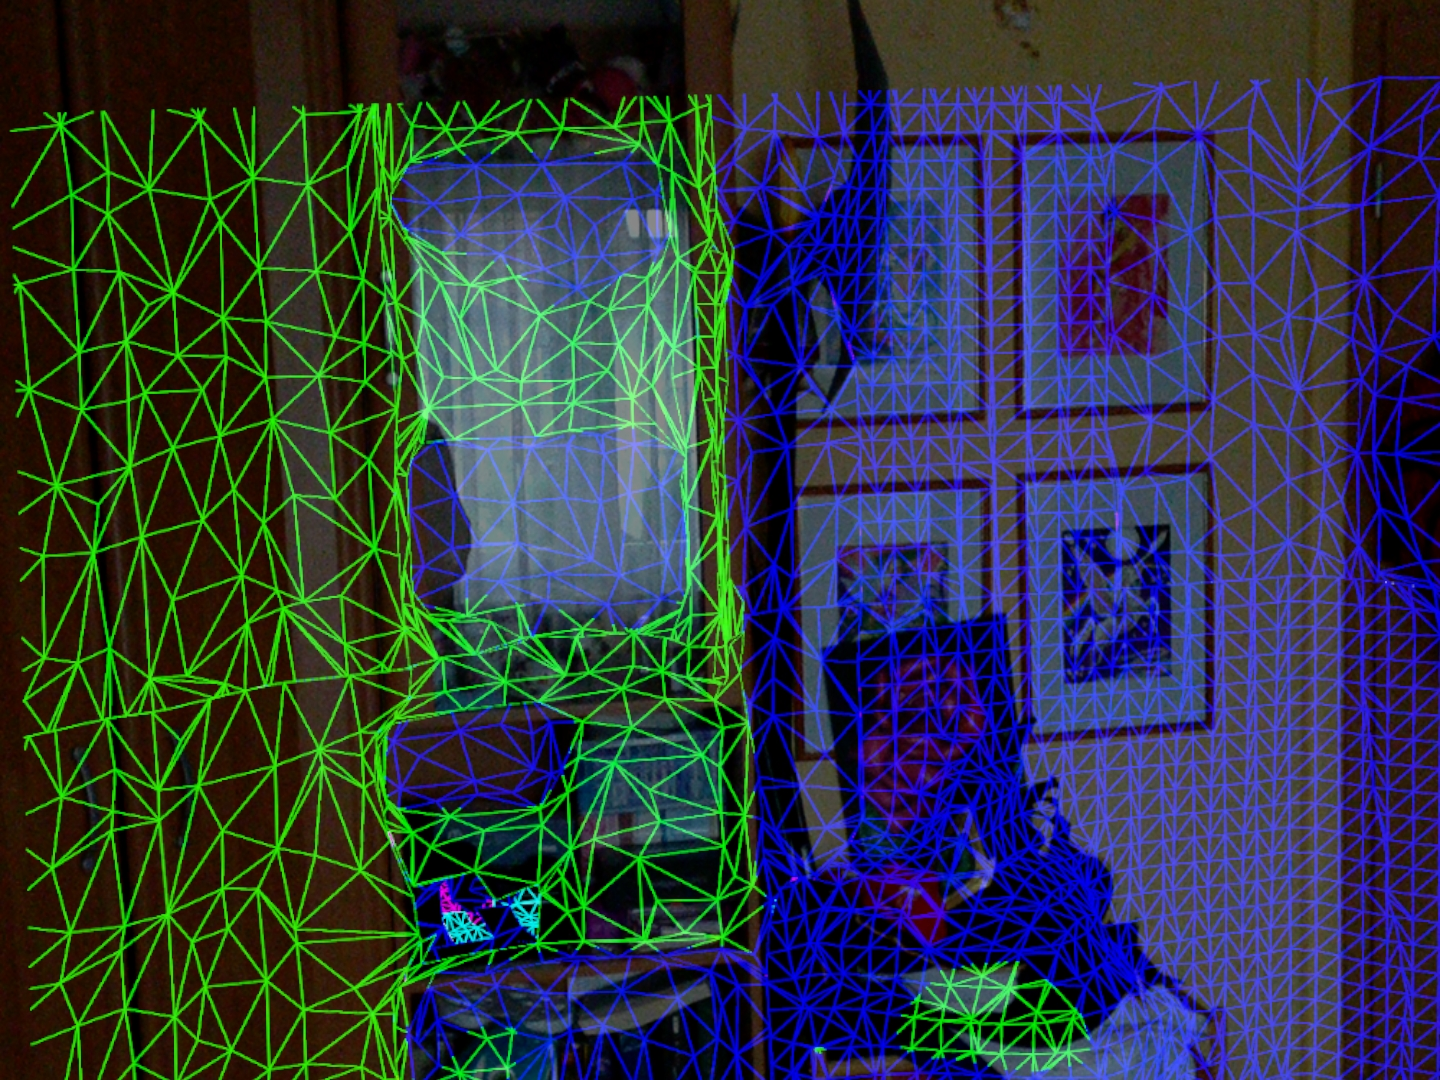
\includegraphics[width=0.7\textwidth]{images/ML_20201003_15.36.42.jpg}
	\caption[Spatial Mapping]{Spatial Map. Die Farben des Meshes zeigen die Entfernung des Nutzers zu den Objekten an.}
	\label{img:spatialmap}
\end{figure}

\subsection{Magic Leap AR Brille}

Die Magic Leap One Lightwear ist eine Augmented Reality Brille, die von dem Unternehmen Magic Leap entwickelt wurde. Sie verfügt über ein Head-Mounted Display und einer Recheneinheit, die über ein Kabel mit dem Display verbunden ist. Die Recheneinheit kann an der Hüfte getragen werden, was die AR Brille mobil macht. 


\subsubsection{Hardware}

Die Recheneinheit besitzt zwei Denver 2.0 64 Bit Prozessor-Kerne und vier ARM Contex A57 46 bit Kerne. Davon ist einer der Denver Kerne und zwei der ARM Contex Kerne für Applikationen nutzbar.  

Sie besitzt neun Sensoren und mehrere Kameras. Dazu gehören:
\begin{itemize}
	\item ein Infrarot Tiefen-Sensor,
	\item ein Eye Tracker,
	\item eine Foto- und Videokamera, die im Format 16:9 mit einer Auflösung von 1920x1080 Pixeln aufnimmt und
	\item mehrere Umgebungskameras die in unterschiedliche Richtungen ausgerichtet sind. \citep{mlofficialsalespitch,mlglossary}
\end{itemize}

Der Output geschieht über ein Display mit einem 50 Grad Field of View und einem Seitenverhältnis von 4:3. Das Display ist transparent. Daher kann die reale Welt immer betrachtet werden. Selbst wenn ein weißes Objekt angezeigt wird, schimmert die reale Welt noch durch. 
Das Display kann keine schwarzen Objekte anzeigen. 

Eingaben erfolgen über einen 6 Degree of Freedom Controller. Er verfügt über 3 Knöpfe (Trigger, Bumper, Home Button) und ein Touchpad. \citep{mlofficialsalespitch,mlglossary}

\begin{figure}[H]
	\centering
	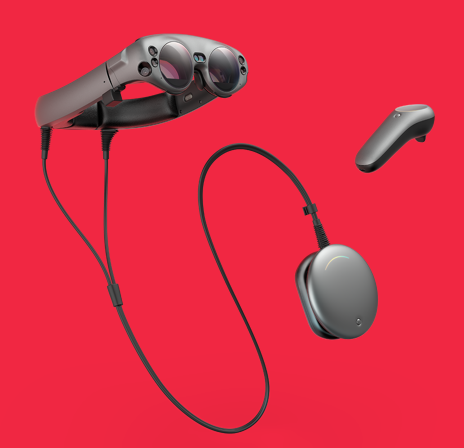
\includegraphics[width=0.7\textwidth]{images/img_magicLeap.PNG}
	\caption[Magic Leap One AR Brille.\citep{mlImage}]{Magic Leap One AR Brille.\citep{mlImage}}
	\label{magcileap}
\end{figure}

\subsubsection{Betriebssystem}
Die Magic Leap Brille läuft auf dem Betriebssystem Lumin OS. Dieses wurde für Augmented Reality entwickelt und bietet Applikationen entsprechende Funktionalitäten an. Beispielsweise führt das Betriebssystem Spatial Mapping durch.\citep{mlluminOS,mlluminfeatures}

Dabei werden mit den Sensoren und Kameras der Brille Daten aufgenommen und in einen zeitlichen Zusammenhang mit der Bewegung der Brille gesetzt, um eine Rekonstruktion des Raumes zu erhalten.\citep{mlluminOS,mlluminfeatures,mlluminworldreconstruktion,mlmeshingunity}

Lumin OS bietet es Applikationen an,
\begin{itemize}
	\item Raycasts auf die Umgebung durchzuführen und
	\item ein Mesh der Rekonstruktion zu erhalten.
\end{itemize}
Neben dem Spatial Mapping unterstützt Lumin OS das Verarbeiten vom Input des Controllers und verwaltet die Zugriffsrechte der Applikationen. Dazu gehört beispielsweise das Recht (Permission) die Fotokamera und das Netzwerk zu nutzen.\citep{mlluminfeatures,mlappsecurity}

Selbst wenn mehrere Applikationen das Recht dazu haben, kann nur eine Applikation zum gleichen Zeitpunkt auf die Fotokamera zugreifen. Die Applikationen müssen sich mit der Kamera-Ressource von Lumin OS verbinden, diese reguliert, welche Applikation Fotoanfragen stellen kann und die aufgenommenen Fotos erhält. 


\subsubsection{Unity Applikationen für Magic Leap One}

Unity ist eine Entwicklungsumgebung, mit der Applikationen für Lumin OS erstellt werden können. Ein Unity Projekt besteht aus mindestens einer Szene, in der mehrere GameObjects existieren. 'GameObject' ist ein Oberbegriff für alle Elemente, die in der Szene existieren. Sie bilden eine hierarchische Struktur, in der GameObjects Parents und Children anderen GameObjects sind.\citep{unitygameobject}

GameObjects haben selbst keine Funktionalität und kein Aussehen. Diese werden durch Components hinzugefügt. Einige Components sind bereits in Unity integriert. Sie geben einem GameObject eine Position in der Szene (Transform Component), machen sie sichtbar (Mesh Renderer) oder gibt dem GameObject die notwendige Logik um als Kamera zu fungieren. Um eine neue Funktionalität zu implementieren, kann ein C\# Script geschrieben werden und einem GameObject als Component zugewiesen werden.

Magic Leap unterstützt die Entwicklung von Applikationen für Lumin OS mit Unity. So wird ein Unity Project Template von Magic Leap angeboten, dass das Set-up der Applikation erleichtert. Dazu gehören Build Optionen und das Einstellen der Hauptkamera der Szene – der Unity Kamera. Die Unity Kamera rendert die Szene für das Display der Magic Leap One. Die Kamera verfolgt die Bewegung der Magic Leap Brille und kopiert diese in der Unity Szene. \citep{mlgetstarted}%Die Szene bleibt somit stationär und die Kamera bewegt sich in ihr, so wie der Nutzer der Magic Leap sich in einer Umgebung bewegt.

Das Unity Template verfügt über vorgefertigte Skripts, die auf Funktionalitäten von Lumin OS zugreifen:

\begin{itemize}
	\item \textit{MLInput} stellt Informationen über den Controller zur Verfügung. Damit können die Knöpfe und Touchpad-Gesten überwacht werden.
	\item \textit{MLCamera} greift auf die Fotokamera der AR Brille zu. Fotoanfragen und Resultat-Daten werden ebenfalls durch MLCamera behandelt.
	\item \textit{MLPrivilegeRequestBehavior} ermöglicht es den Nutzer nach dem Recht zu fragen, auf bestimmte Teile des AR Systems zuzugreifen. Beispielsweise muss nach Permission gefragt werden, um die Fotokamera-Ressource zu verwenden. 
	\item \textit{MLRaycast} greift auf die Spatial Mapping Funktionalitäten von Lumin OS zu. Es gibt einen Raycast auf die Rekonstruktion der Umgebung beim Betriebssystem in Auftrag. 
	\item \textit{MLSpatialMapper} zeigt die Rekonstruktion der Umgebung von Lumin OS als Mesh an. Das Mesh besteht aus GameObjects, die von \textit{MLSpatialMapper} erzeugt werden. Sie werden ständig aktualisiert, um das geometrische Verständnis des Betriebssystems wiederzuspiegeln.
\end{itemize}

Scripts können von der Klasse \textit{Monobehavior} erben. \textit{Monobehaviors} verfügen über Methoden, die von Unity zu unterschiedlichen Events der Laufzeit ausgeführt werden. Nur Skripts, die ein Component eines GameObjects sind, werden aufgerufen.

\begin{itemize}
	\item \textit{Awake} - diese Methode wird aufgerufen, wenn das GameObject initialisiert wird. %Wenn ein GameObject initialisiert wird, werden die Awake() Methoden der Componenten aufgerufen.
	\item \textit{Update} - die Update Methoden der Scripts werden zu jedem Frame aufgerufen.
	\item \textit{OnDestroy} - diese Methode wird aufgerufen, wenn das GameObject aus der Szene gelöscht wird.
\end{itemize}

\textit{Monobehaviors} können über globale Variablen verfügen. Wenn das Skript einem GameObject als angehören, kann der Inhalt der globalen Variable in Unity modifiziert werden. Dadurch kann einem Skript eine Referenz auf ein bestimmtes GameObject gegeben werden. Siehe Abbildung \ref{img:gloabvars}.

\begin{figure}[H]
	\centering
	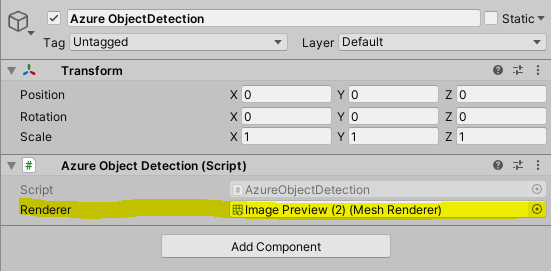
\includegraphics[width=0.8\textwidth]{images/img_globalVars.png}
	\caption[Unity GameObject mit Components]{GameObject mit Components. Die Component Azure Object Detection verfügt über eine globale Variable (in gelb), die auf eine Mesh Renderer Component eines anderen Objektes verweist.}
	\label{img:gloabvars}
\end{figure}


\textit{Monobehaviors} können als Singleton fungieren, indem sie eine globale statische Referenz auf sich selber anlegen, wenn ihre \textit{Awake} Methode aufgerufen wird.%Siehe Abbildung \ref{code:singleton}.

\begin{lstlisting}
public class MySingletonClass : MonoBehavior
{
	public static MySingletonClass instance = null;
	private void Awake()
	{
		if (instance != null && instance != this)
		{
			Destory(this.gameObject);
		}
		instance = this;
	}
	public void DoSomething(){...}
}
\end{lstlisting}

%\begin{figure}[H]
%	\centering
%	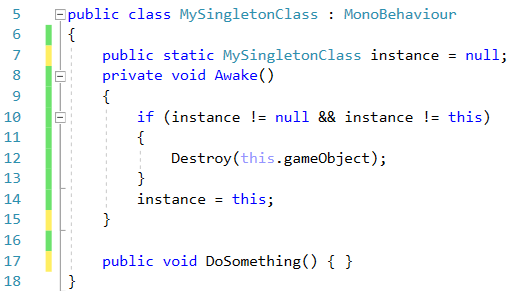
\includegraphics[width=0.7\textwidth]{images/code_singleton.png}
%	\caption[Quellcode Singleton Klasse]{Quellcode einer Singleton Klasse}
%	\label{code:singleton}
%\end{figure}

Jedes andere Script kann die Instanz des Singletons aufrufen, indem es die statische Referenz der Klasse des Singletons verwendet. %Siehe Abbildung \ref{code:singleton2}.
\begin{lstlisting}
MySingletonClass.instance.DoSomething();
\end{lstlisting}
%\begin{figure}[H]
%	\centering
%	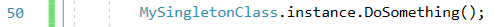
\includegraphics[width=0.7\textwidth]{images/code_singleton2.png}
%	\caption[Quellcode Aufrug des Singletons]{Quellcode Aufruf des Singletons}
%	\label{code:singleton2}
%\end{figure}

Skripts können während der Laufzeit GameObjects erzeugen. Um festzulegen, wie das GameObject aussehen soll, kann in dem Unity Editor ein Prefab erstellt werden. Prefabs sind vorgefertigte, abgespeicherte GameObjects, deren Child Objects, Components und globale Variablen festgelegt werden. Das Prefab fungiert als Vorlage für GameObjects die zur Laufzeit initialisiert werden. Während der Initialisierung wird eine Position der Szene angegeben, an die das neue GameObject gesetzt wird. Nachdem das Objekt initialisiert wurde, kann auf seine Components und Scripts zugegriffen werden.\citep{unityprefabs}


\subsubsection{Lokale und globale Koordinatensysteme in 3D Szenen}
%\newline
In der 3D Szene werden die Positionen von Objekten als Matrizen in dreidimensionalen Koordinatensystemen verwaltet. Es gibt ein globales Koordinatensystem (auch Weltkoordinatensystem oder World Space), in dem alle Objekte relativ zu einem Ursprung liegen. 

Jedes Objekt hat zusätzlich ein eigenes, lokales Koordinatensystem (Objektkoordinatensystem). Dessen Ursprung liegt in dem jeweiligen Objekt. Die Position und Rotation des Objektes in dem globalen Koordinatensystem bestimmt die Relation zwischen dem globalen und dem lokalen Koordinatensystem. 

Das lokale Koordinatensystem einer Kamera wird auch Camera Space genannt. Die Relation zwischen dem Camera Space und dem globalen Koordinatensystem wird in Unity durch die \textit{cameraToWorld} Matrix beschrieben. Mithilfe dieser Matrix kann eine Koordinate aus dem Camera Space in die entsprechende Koordinate des globalen Koordinatensystems transformiert werden. Dazu wird die Koordinate als Vektor angegeben und mit der cameraToWorld Matrix multipliziert. Das Resultat ist ein Vektor, der eine Koordinate im globalen Koordinatensystem angibt.\citep{unitycameratoworldmatrix,unitymultiplyoint}

\subsubsection{Kamera in 3D-Computergrafik}
\paragraph{View Frustum}
ist das Teilvolumen einer 3D Szene, die auf einen zweidimensionalen Bildschirm abgebildet wird. Alle Objekte, die von der Kamera gesehen werden, befinden sich in dem View Frustum.

\paragraph{Clipping Plane}
bezeichnet eine Ebene, die den View Frustum quer zur Blickrichtung begrenzt. Es gibt eine vordere und eine hintere Clipping Plane. Die vordere Clipping Plane liegt nah an der Kamera. Alle Objekte die zwischen der Kamera und der vorderen Clipping Plane liegen, werden nicht angezeigt. Die hintere Clipping Plane limitiert wie weit Objekte entfernt sein können, bevor sie nicht mehr zu sehen sind. Siehe Abbildung \ref{dia:clipping}.\citep{unityclipping}

\begin{figure}[H]
	\centering
	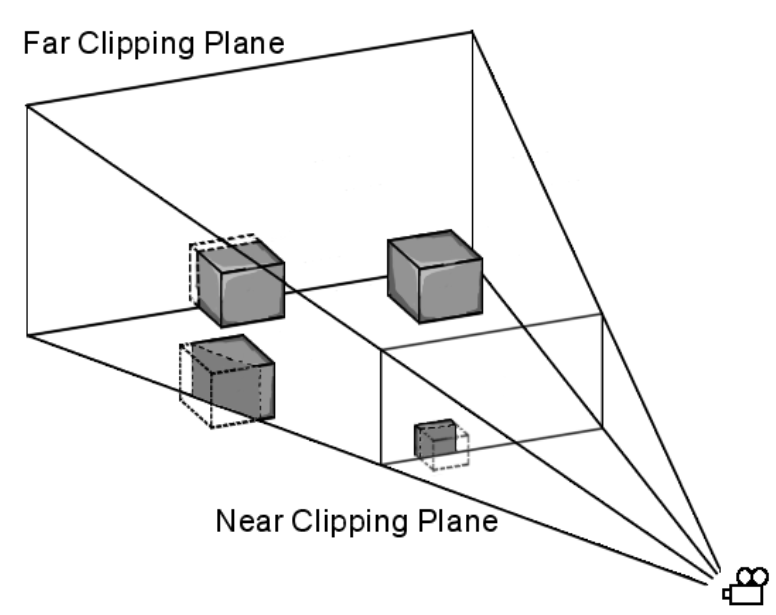
\includegraphics[width=0.7\textwidth]{images/dia_ViewFrustum.png}
	\caption[View Frustum]{Diagramm des View Frustum mit Clipping Planes.}
	\label{dia:clipping}
\end{figure}

%to myself: yay :) you're doing well I believe in you!

\subsection{Computer Vision}
Computer Vision setzt das Ziel die Inhalte digitaler Bilder und Videos zu verstehen. Sowohl semantische als auch geometrische Inhalte werden dabei analysiert. 
Zu den Aufgaben von Computer Vision gehören: Objekterkennung, Bild-Segmentierung, Menschen erkennen und Bewegungen in Videos nachverfolgen.

In diesem Feld kommen Statistik, Bilderverarbeitung und Maschinelles Lernen zum Einsatz. Maschinelles Lernen wird eingesetzt, um neuronale Netze zu formen, die Bild- und Videoanalysen durchführen können.\citep{intortodeeplearingmedical}

\subsubsection{Object Detection}

Objekt Detection ist eine Aufgabe der Computer Vision. Es sollen mehrere Objekte in einem Bild erkannt werden. Daher wird es auch Image Based Object Detection genannt. Spezialisierungen von Object Detection sind beispielsweise Gesichtserkennung oder das Erkennen von Fußgängern. Durch eine Objekterkennung werden semantische Inhalte eines Bildes automatisch erhoben. 

Für die Objekte wird eine Klasse und eine Bounding Box bestimmt. Die Klasse gibt an, um welche Art von Objekt es sich handeln. Beispielsweise ob es eine Tastatur oder ein Computerbildschirm ist (Object Classification). Die Bounding Box gibt ein Viereck in dem Bild an, in dem sich das Objekt befindet(Object Localization). \citep{objectdetection,objectDetectionReview}



%todo Eventuell kannst du auch noch kurz was zur objekterkennung dort einpacken (das sind allerdings schon sehr alte paper ;) Das letzte geht aber auch im 3.3.1
\subsubsection{Artificial Neural Networks}
Artificial Neural Networks sind Machine Learning Architekturen. Sie können beispielsweise Musik, Text oder Bilder nach Mustern durchsuchen. Sie sind für keine genaue Aufgabe programmiert, sondern lernen indem sie mit Beispieldaten trainiert werden. Für jedes Beispiel gibt es ein Label, das angibt, ob es das gesuchte Muster enthält oder nicht. Die Struktur des Networks verfügt über Gewichte, die Einfluss auf den Output haben. Mit jedem Trainingsbeispiel passt das Network die Gewichte an, sodass der Output dem Label des Beispiels entspricht.\citep{introToCNN,surveyOfDeepLearing}

Artificial Neural Networks bestehen aus einer Menge an verbundenen Knoten, die jeweils eine Berechnung durchführen. Diese Knoten sind in Ebenen aufgeteilt, den Input Layer, den Output Layer, und mehrere Hidden Layer dazwischen. Die Knoten einer Ebene sind mit allen Knoten der vorherigen Ebene verbunden.\citep{introToCNN,surveyOfDeepLearing}

Das Neural Network bekommt eine Menge an Daten als Input. Die Knoten arbeiten zusammen, um den Output zu erzeugen. Dabei wird über Gewichte entschieden, wie viel Einfluss das Ergebnis der einzelnen Knoten auf die nächste Ebene hat.\citep{introToCNN,surveyOfDeepLearing}

Um ein Neural Network zu trainieren, wird der Output von einem Mensch bewertet. Das Neural Network nutzt diese Bewertung, um die Gewichte der einzelnen Knoten zu verändern. So passt sich das Neural Network an. \citep{introToCNN,surveyOfDeepLearing}

\subsubsection{Convolutional Neural Networks}
Convolutional Neural Networks sind auf das Verarbeiten von Bildern spezialisiert. Sie nutzen aus, das Bilder viele Redundanzen und informationsarme Bereiche haben. Daher können mit jedem Verarbeitungsschritt des Networks Informationen weggelassen werden. So können Rechenzeit und Volumen der Trainingsdaten verringert werden.\citep{introToCNN,surveyOfDeepLearing,cNNforClass}

Convolutional Neural Networks sind Machine Learning Architekturen, die darauf ausgelegt sind, Muster in Bildern zu erkennen. Sie müssen auf das Muster trainiert werden. Dazu wird ihnen eine Menge an Bildern, die Teilweise das Muster erhalten, und der gewünschte Output, der erreicht werden soll, gegeben. Die Struktur des Network verfügt über Gewichte, die die Berechnung des Outputs beeinflussen. Mit jedem Trainigsbild passt das Network die Gewichte an, damit es die Muster korrekt erkennen kann.\citep{introToCNN,surveyOfDeepLearing}

Convolutional Neural Networks werden hauptsächlich eingesetzt, um Muster in Bildern zu erkennen. Daher ist ihre Struktur und ihre Arbeitsweise auf Bilder spezialisiert. Sie brauchen weniger Rechenzeit und weniger Trainingsdaten als ein generelles Artificial Neural Network für dieselbe Aufgabe brauchen würde.\citep{introToCNN,surveyOfDeepLearing,cNNforClass} 

Die Knoten in einer Ebene eines Convolutional Neural Network sind nur mit wenigen Knoten der vorherigen Ebene verbunden. So sinkt die Menge an Informationen mit jeder Ebene. Das CNN wird gezwungen sich auf wesentliche Teile des Bildes zu konzentrieren, mit denen beispielsweise ein Objekt oder  Muster erkannt werden kann. \citep{introToCNN,surveyOfDeepLearing}

\subsubsection{Azure Computer Vision Services}

Microsoft Azure ist eine Cloud Computing Plattform von Microsoft. Seit 2010 stellt sie Cloud Services zur Verfügung, die unter andrem Computer Vision Aufgaben durchführen. 
Diese sind über REST APIs erreichbar. 

Rest steht für Representational State Transfer. Eine Rest API ist eine Programmierschnittstelle, die sich an dem Verhalten des World Wide Web orientiert. Die Kommunikation zwischen einem Client und dem Server orientiert sich an REST.
Rest steht für Representation State Transfer und bezeichnet einen Architekturansatz wie verteile Systeme miteinander kommunizieren können. REST verlangt unter anderem ein Client-Server Modell und zustandslose Kommunikationen zwischen ihnen. Jede Anfrage eines Clients beinhaltet alle Informationen, die der Server benötigt um sie zu beantworten. %rest is just an idea. describe it a bit more

Eine Rest-API kann mit http/s realisiert werden. Der Server / Service kann durch eine URL angesprochen werden. Diese wird auch Endpoint genannt. HTTP-Methoden, wie GET und POST kommunizieren an den Service welche Operation durchgeführt werden soll. Diese werden auch Http-Anfragen oder HTTP Request genannt. Mit Get werden Daten von dem Server angefordert. Die Post Methode erlaubt das Übermitteln von zusätzlichen Daten an der Server.

Ein HTTP Request besteht aus einer Start Line, einer Menge an Headers und einem Body. Die Start Line gibt die HTTP-Methode (GET, POST, ...) und eine Endpoint-URL an.
In den Headers werden weitere Informationen über die Anfrage an den Server angegeben. Für die Anwendung einer API, wird Authentifizierungsschlüssel des Clients in einem Header gespeichert.
Zuletzt hat der Request einen Body. Abhängig von der HTTP-Methode beinhaltet der HTTP-Request Daten für den Server. So speichert eine POST Nachricht ihre Daten, beispielsweise ein Foto, in dem Body. Die Länge und Art der Daten wird mit Headern angegeben.
  
Auf jede HTTP-Anfrage wird eine HTTP-Response als Antwort zurückgeschickt. 
Die HTTP-Response besteht ebenfalls aus einer Start Line, Headern und einem Body. Die Start Line gibt einen Response Code und einen Statustext an. Der Response Code teilt dem Client mit, ob die Anfrage erfolgreich bearbeitet wurde. Wenn ein Error aufgetreten ist, gibt der Statuscode Auskunft über die Art des Errors. Der Statustext gibt eine kurze Erklärung des Response Codes.

Beispiel Response Codes:
\begin{itemize}
	\item 404 - Url nicht gefunden
	\item 401 - Zugriff verweigert wegen ungültiger Authentifizierung
	\item 400 - fehlerhafte Anfrage. Der Service konnte die Anfrage nicht verstehen
	\item 200 - Anfrage wurde erfolgreich bearbeitet
\end{itemize}

Eine API schickt, bei einer erfolgreichen Bearbeitung der Anfrage, in dem Body der HTTP-Response die erfragten Daten mit.

\subsubsection{Azure Object Detection}
Microsoft Azure bietet einen Computer Vision Service an. Dabei handelt es sich um mehrere KIs, die für unterschiedliche Aufgaben trainiert wurden. Dazu gehört unter anderem ein Service für Object Detection. Dabei sendet der Anwender ein Bild an Microsoft, dort wird es verarbeitet und ein Ergebnis in Form einer Json Datei zurückgeschickt.\citep{getAzure,whatIsAzure,objDetectAzure,Azure302Doc}

Die Object Detection basiert auf einem trainierten KI-Modell. Dieses kann nur Objekte erkennen, für die es trainiert wurde. Zusätzlich können Objekte, die in dem Foto sehr klein sind oder nah bei anderen Objekten liegen, nicht erkannt werden.\citep{azureobjdetec}

Der Service ist durch eine REST-API erreichbar. Mit einer Post Anforderung werden die Bilddaten übertragen und die Analyse angefragt. Die Response Nachricht beinhaltet eine Json-Datei, welche die gefundene Objekte und deren Positionen auf dem Foto beinhaltet. Um den Service zu nutzen wird eine Http Post Anforderung an die Webadresse geschickt. Als Endpoint wird die Webadresse der REST-API angegeben. Die Nachricht muss folgenden Inhalt haben:
\begin{itemize}
	\item Ein Authentifizierungsschlüssel, der mit einem Azure Account verbunden ist
	\item und Bilddaten
\end{itemize}

Das Resultat der Analyse wird in der Response-Nachricht zurückgeschickt. Der Response Code 200 gibt an, das die Analyse durchgeführt wurde. In diesem Falle wird eine Json Datei mitgeschickt. Beispielhaft:

\begin{lstlisting}
{"objects":[{"rectangle":{"x":1377,"y":900,"w":157,"h":138},"object":"computer mouse","confidence":0.681},
{"rectangle":{"x":1336,"y":0,"w":584,"h":841},"object":"display","confidence":0.873},
{"rectangle":{"x":315,"y":25,"w":906,"h":622},"object":"display","confidence":0.839},
{"rectangle":{"x":447,"y":800,"w":862,"h":166},"object":"computer keyboard","confidence":0.71}],
"requestId":"a77e261a-7d40-4159-bf78-19d8fb61ad92",
"metadata":{"height":1080,"width":1920,"format":"Jpeg"}}
\end{lstlisting}

Die gefundenen Objekte befinden sich in der Liste mit dem Key 'objects'. Jedes Element der Liste hat ein Bounding Box 'rectangle' und eine Klassenbezeichnung 'object'. Zusätzlich hat jedes Object einen 'confidence' Score. Dieser gibt die Wahrscheinlichkeit an, das das Objekt korrekt erkannt wurde. 
Neben den Objekten wird noch eine requestId und Metadaten über das Bild zurückgeschickt.

\subsubsection{Azure Custom Vision}
Azure bietet zusätzlich einen Computer Vision Service an, den der Nutzer trainieren kann. 
Das verwendete KI-Modell ist für Objekt Detection entwickelt und ist untrainiert.
Custom Vision kann als Ergänzung zu Azure Object Detection verwendet werden.\citep{Azure302bDoc}

Das KI-Modell lässt sich für Image Klassifizierung oder Objekt Detection trainieren. Über eine Webseite lässt sich der Trainingsprozess des Modells steuern und auswerten. Der Nutzer lädt Fotos hoch und fügt jedem Foto händisch einen oder mehrere Tags hinzu. Die Tags geben die Objekt-Klasse an, die sich in dem Bild befindet. Um das Modell für Object Detection zu trainieren, kann eine rechteckige Region in dem Foto markiert werden, um das Objekt zu lokalisieren. Siehe Abbildung \ref{img:trainingone}. In einem Bild können mehrere Regionen markiert werden. Jede Region wird mit einem Tag annotiert.

\begin{figure}[H]
	\centering
	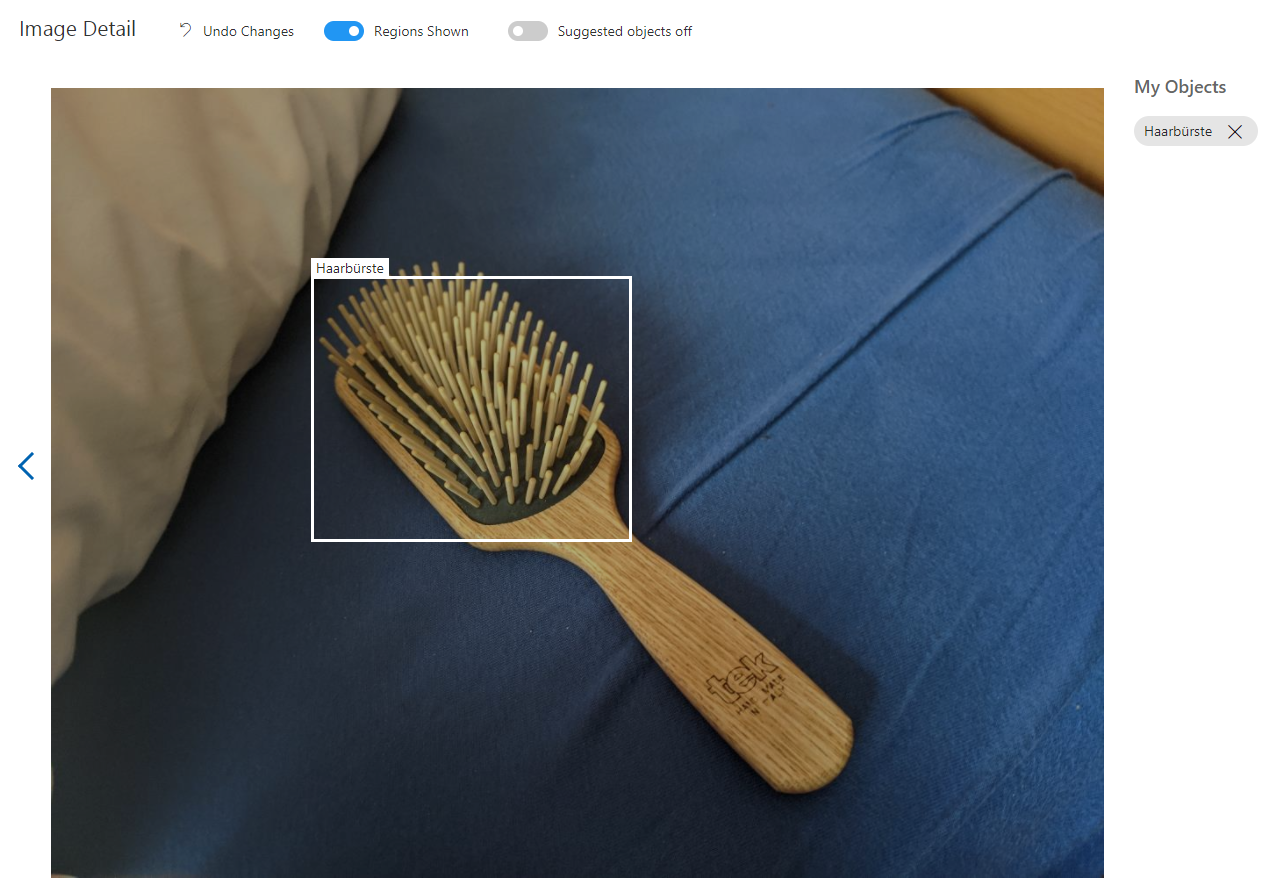
\includegraphics[width=1\textwidth]{images/trainingone.png}
	\caption[Trainingsbild für Azrue Custom Detection]{Trainingsbild für die Objekterkennung einer Haarbürste.}
	\label{img:trainingone}
\end{figure}

Für jede Objekt-Klasse müssen mindestens 15 Bilder hochgeladen werden, in denen der entsprechende Tag vorkommt. Nur dann kann der Trainingsprozess gestartet werden. Mit mehr Bildern in dem Trainingsset wird die Objekterkennung des Modells jedoch robuster. Azure empfehlt es mindestens 50 Bilder pro Tag zu verwenden. Wenn mit nur wenigen Bildern trainiert wird, haben die einzelnen gewählten Bilder einen sehr großen Einfluss auf das Modell.

Durch das Trainieren wird eine Iteration des Modells erzeugt. Diese Iteration kann verwendet werden, um Object Detection durchzuführen. Wird erneut der Trainingsprozess gestartet, wird eine weitere Iteration erstellt. Die Iterationen werden alle unter einer Projekt ID gespeichert. Die Iterationen des Modells werden in einer Testphase evaluiert. Für jede Objekt-Klasse werden drei Metriken angesetzt. 
\begin{itemize}
	\item Precision - die Wahrscheinlichkeit das ein gefundenes Objekt, tatsächlich der angegeben Klasse angehört. (Die Wahrscheinlichkeit das es kein false positive ist.)
	\item Recall - aus einer Menge an Objekten die einer Klasse angehören, der Prozentsatz an Objekten, die das Modell korrekt lokalisieren und klassifizieren konnte.
	\item a.p (Average Precision) - eine Gesamtwertung für die Evaluierung basierend auf Precision und Recall. 
\end{itemize}

Die Evaluierungen der einzelnen Objekt-Klassen werden in Precision, Recall und mean Average Percision gemittelt. Siehe Abbildung  \ref{img:trainineval}.

\begin{figure}[H]
	\centering
	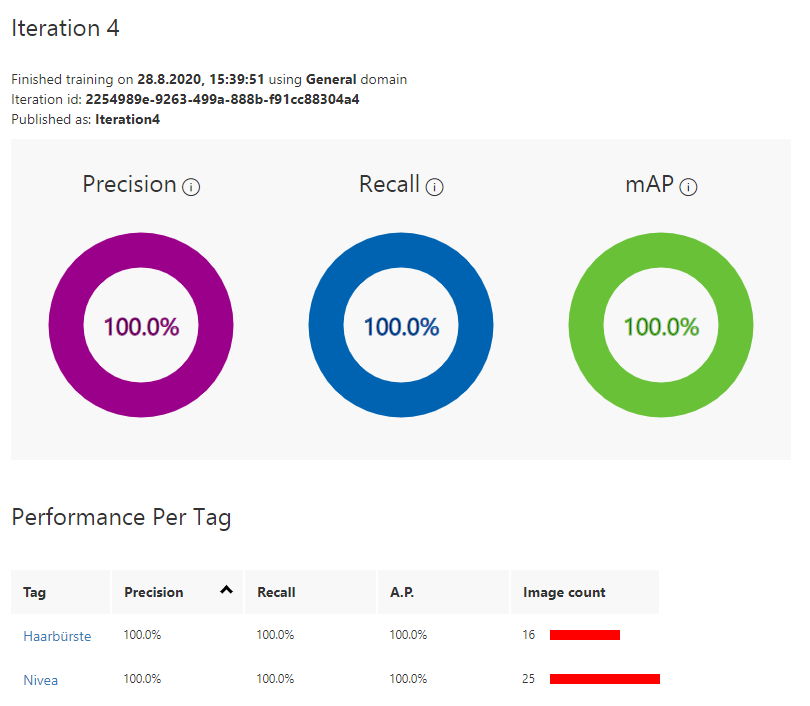
\includegraphics[width=1\textwidth]{images/trainingevaluation.png}
	\caption[Evaluierung eines Azure Custom Detection Modells]{Die Evaluierung des Modells}
	\label{img:trainineval}
\end{figure}

Mit einer erzeugten Iteration des Modells können Fotos auf Objekte untersucht werden. Genauso wie Azure Object Detection ist das Custom Modell durch eine REST-API erreichbar. 
Der Endpoint beinhaltet die ID des Projektes, und die Nummer der Iteration, die verwendet werden soll.
In der Post Nachricht wird ein Authentifizierungsschlüssel und ein zu analysierendes Bild mitgeschickt.

Das Resultat der Analyse ist eine Json Datei. 
Der Aufbau der Datei unterscheidet sich vom Dateiaufbau von Azure Object Detection leicht. Informationen über die Iteration, die für die Analyse verwendet wurde, werden wiedergegeben. 

\begin{lstlisting}
{"id":"9cb0cc50-1dca-4b4a-b4d1-95d6bd25c352",
"project":"ac915246-5268-461f-bd11-cf0c1826d509",
"iteration":"2254989e-9263-499a-888b-f91cc88304a4",
"created":"2020-10-10T02:40:40.107Z",
"predictions":[{"probability":0.997380137,"tagId":"d390d34e-afc4-4ff4-8dcd-3ee8fe79cb8f","tagName":"Haarbürste","boundingBox":{"left":0.258805573,"top":0.226171583,"width":0.303168833,"height":0.329167157}},
{"probability":0.0141124222,"tagId":"d390d34e-afc4-4ff4-8dcd-3ee8fe79cb8f","tagName":"Haarbürste","boundingBox":{"left":0.542580664,"top":0.507969,"width":0.2195471,"height":0.3491398}},
{"probability":0.0116642443,"tagId":"263b3042-8958-4775-9a19-e2602d19c9b7","tagName":"Nivea","boundingBox":{"left":0.542580664,"top":0.507969,"width":0.2195471,"height":0.3491398}}]}
\end{lstlisting}

Die gefundenen Objekte werden in der Liste "predictions" aufgezählt. Die Objektklassen werden in "tagName" gespeichert. Die "probability" gibt das Vertrauen des Modells darin an, dass das Objekt korrekt erkannt wurde. Die erkannten Objekte müssen bei nach ihrer Probability gefiltert werden, da auch Objekte mit einer sehr niedrigen Probability in der Json Datei enthalten sind. 